\subsubsection{Caso d'uso UC8.1.3.7: Creazione domanda con area cliccabile nell'immagine}
\label{UC8.1.3.7}
\begin{figure}[h]
	\centering
	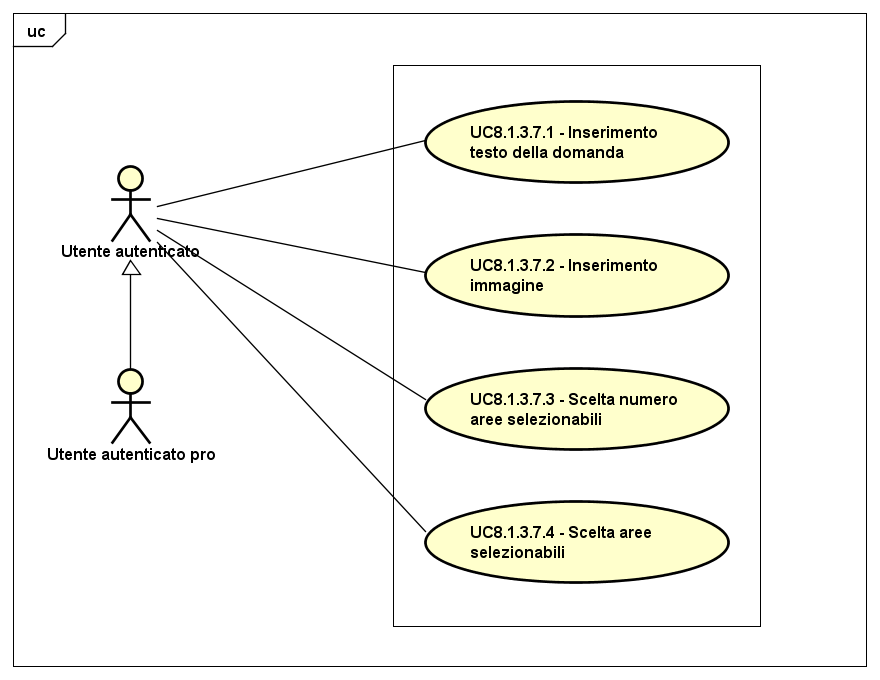
\includegraphics[scale=0.5,keepaspectratio]{UML/UC8_1_3_7.png}
	\caption{UC8.1.3.7: Creazione domanda a risposta multipla}
\end{figure}
\FloatBarrier
\begin{itemize}
	\item \textbf{Attori}: utente autenticato, utente autenticato pro;
	\item \textbf{Descrizione}: questa funzionalità offre agli attori la possibilità di creare domande la cui risposta è selezionabile all'interno di aree cliccabili in un immagine;
	\item \textbf{Precondizione}: gli attori hanno selezionato la seguente funzionalità; 
	\item \textbf{Postcondizione}: gli attori hanno creato una domanda con area cliccabile nell'immagine;
	\item \textbf{Scenario principale}:
		\begin{enumerate}
	       	\item Gli attori possono compilare il campo dati destinato alla scrittura del testo della domanda (UC8.1.3.7.1);
	        \item Gli attori possono inserire una immagine relativa al testo della domanda (UC8.1.3.7.2);
			\item Gli attori possono scegliere quante aree saranno selezionabili all'interno dell'immagine (UC8.1.3.7.3);
			\item Gli attori possono scegliere le aree selezionabili all'interno dell'immagine (UC8.1.3.7.4);
	 	\end{enumerate}
\end{itemize}

\subsubsection{Caso d'uso UC8.1.3.7.1: Compilazione testo domanda}
\begin{itemize}
	\item \textbf{Attori}: utente autenticato, utente autenticato pro;
	\item \textbf{Descrizione}: gli attori possono inserire un testo per la domanda che vogliono creare;
	\item \textbf{Precondizione}: gli attori hanno selezionato la modalità di creazione di una domanda con area cliccabile;
	\item \textbf{Postcondizione}: gli attori hanno inserito il testo della domanda.
\end{itemize}

\subsubsection{Caso d'uso UC8.1.3.7.2: Inserimento immagine}
\begin{itemize}
	\item \textbf{Attori}: utente autenticato, utente autenticato pro;
	\item \textbf{Descrizione}: gli attori hanno la possibilità di inserire un'immagine relativa al testo della domanda;
	\item \textbf{Precondizione}: gli attori hanno selezionato la modalità di creazione di una domanda con area cliccabile; 
	\item \textbf{Postcondizione}: gli attori hanno inserito l'immagine;
	\item \textbf{Scenario principale}: gli attori inseriscono l'immagine. 	
\end{itemize}

\subsubsection{Caso d'uso UC8.1.3.7.3: Scelta numero aree selezionabili}
\begin{itemize}
	\item \textbf{Attori}: utente autenticato, utente autenticato pro;
	\item \textbf{Descrizione}: gli attori hanno la possibilità di scegliere il numero di aree selezionabili all'interno dell'immagine;
	\item \textbf{Precondizione}: gli attori hanno selezionato la modalità di creazione di una domanda con area cliccabile; 
	\item \textbf{Postcondizione}: gli attori hanno scelto il numero di aree selezionabili all'interno dell'immagine;
	\item \textbf{Scenario principale}: gli attori scelgono il numero di aree selezionabili all'interno dell'immagine. 	
\end{itemize}

\subsubsection{Caso d'uso UC8.1.3.7.4: Scelta aree selezionabili}
\begin{itemize}
	\item \textbf{Attori}: utente autenticato, utente autenticato pro;
	\item \textbf{Descrizione}: gli attori hanno la possibilità di scegliere le aree selezionabili all'interno dell'immagine;
	\item \textbf{Precondizione}: gli attori hanno selezionato la modalità di creazione di una domanda con area cliccabile; 
	\item \textbf{Postcondizione}: gli attori hanno scelto le aree selezionabili all'interno dell'immagine;
	\item \textbf{Scenario principale}: gli attori scelgono le aree selezionabili all'interno dell'immagine. 	
\end{itemize}

